\section{Bag of Visual Words}
Local feature extractors provide us with varied number of descriptors for each image. However, for classification, we need each image to be represented by a single vector. This can be achieved using a Bag of Words technique.

Bag of Words (BoW) is a technique, which represents each sample in a dataset as a multiset of its words. In general, these words do not have to be literal words but can be any categorization of information provided by the sample.

First BoW needs to generate a dictionary. The dictionary is a set of $k \in \mathbb{N}$ categories of words called bins. The BoW then assigns each word to a bin. Finally, for each sample in the dataset, a histogram of amounts of words belonging to each bin is created.

We explain the technique with text documents as samples. With text documents, the dictionary consists of every unique word in all documents. The words of each document are assigned to a bin of said words.

For example, in a dictionary consisting of bins \{ \say{Peter}, \say{run}, \say{talked}, \say{to} \}, a sample sentence \say{Peter talked to Peter} would produce the following histogram:
\begin{equation}
    \{2, 0, 1, 1\}.
\end{equation}

In our case, we consider the descriptors found in an image as words. As we are dealing with visual information, let us call these words \say{visual words} and nickname the BoW technique \say{Bag of Visual Words} (BoVW).

We generate the categories using a $k$-means algorithm on all the visual words in the training dataset. We then assign the visual words to the closest (considering euclidean distance) category.

\subsection{$k$-means}
The $k$-means algorithm is an unsupervised learning technique. Let $X=\{ x_1, x_2, \dots, x_n \}$ be a dataset of $n$ data-points. The goal is to sort the data points into $k$ clusters $S = \{ S_1, S_2, \dots, S_k \}$, such that
\begin{equation}
    \argmin_S \sum_{i=1}^k \sum_{x\in S_i} \norm{x-c_i}^2,
\end{equation}
where \(c_1, c_2, ..., c_k \) are the centroids of \(S_1, S_2, ..., S_k \), respectively. The centroids are determined as means of data points belonging to each cluster.

The algorithm starts by selecting $k$ random data points as the centroids. Then alternates between these two steps until a terminate condition is met:
\begin{description}
    \item{\textbf{Assignment step:}} Each data point is assigned to the cluster, such that the Euclidean distance between the centroids of the clusters and the current data point is the smallest one.
    \item{\textbf{Update step:}} For each cluster, a new centroid is computed as the mean of data points belonging to this cluster.
\end{description}

The terminate condition is met, when the ratio of the samples, for which the assigned cluster changes, to the total amount of samples, is smaller than a specified threshold. The steps of the algorithm can be seen in \figref{fig:k_means_alg}.
\begin{figure}[ht]
    \centering
    \begin{subfigure}[t]{0.22\textwidth}
        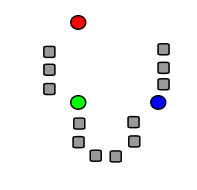
\includegraphics[width=\textwidth]{Figures/k-means/k-means_inicial_step.png}
        \caption{At first, random data points are selected as the initial $k$ centroids.}
        \label{fig:k-means-alg:inicial_step}
    \end{subfigure}\hfill
    \begin{subfigure}[t]{0.22\textwidth}
        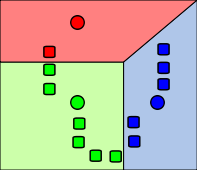
\includegraphics[width=\textwidth]{Figures/k-means/k-means_assignment_step.png}
        \caption{By choosing the nearest centroid, each data point is assigned its cluster.}
        \label{fig:k-means-alg:assignment_step}
    \end{subfigure}\hfill
    \begin{subfigure}[t]{0.22\textwidth}
        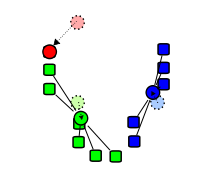
\includegraphics[width=\textwidth]{Figures/k-means/k-means_update_step.png}
        \caption{New centroids are calculated as means of data points in the cluster.}
        \label{fig:k-means-alg:update_step}
    \end{subfigure}\hfill
    \begin{subfigure}[t]{0.22\textwidth}
        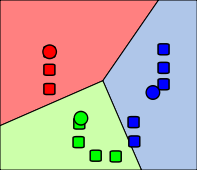
\includegraphics[width=\textwidth]{Figures/k-means/k-means_assignment_step_2.png}
        \caption{Steps in (b) and (c) are repeated until the terminate condition is met.}
        \label{fig:k-means-alg:assignment_step_2}
    \end{subfigure}\hfill
    \caption[Lloyd's algorithm demonstration.]{Lloyd algorithm demonstration. \cite{Wikikmeans}}
    \label{fig:k_means_alg}
\end{figure}
The challenge is determining the $k$ number of clusters, and therefore the size of the visual dictionary. In our experiments, we try different settings for $k$ to find a clustering, which best represents our data.
